\section{Algorithm}
	
	\begin{figure}[ht!]
		\hspace*{-1.8cm}
		\begin{tikzpicture}
			[node distance=1.5cm]
			
			\tikzstyle{startstop} = [rectangle, rounded corners, minimum width=3cm, minimum height=1cm,text centered, draw=black, fill=pink!30,align = center]
			
			\tikzstyle{io} = [trapezium, trapezium left angle=70, trapezium right 	angle=110, minimum width=3cm, minimum height=1cm, text centered, draw=black]
			
			\tikzstyle{process} = [rectangle, minimum width=3cm, minimum height=1cm, text 	centered, draw=black,align = center, fill = blue!20]
			
			\tikzstyle{decision} = [diamond, minimum width=3cm, minimum height=1cm, 
			align = center, draw=black, fill = green!20]
						
			\tikzstyle{arrow} = [thick,->,>=stealth]

			\node (st) [startstop] {Start};
			\node (pls) [process,below of=st] {Pulse leds};
			\node (wt) [process, below of=pls] {Wait 0.5 secs};
			\node (findlv) [decision, below of=wt,yshift=-1cm] {$V_1$ within\\preset levels};
			\node (setlv) [process, left of=findlv,xshift=-3cm] {Set new drive current};
			\node (dc) [process, below of=findlv,yshift=-1cm] {Find red/ir \\DC levels};
			\node (diff) [process, below of=dc] {Generate Diff signal};
			\node (amp) [decision, below of=diff,yshift=-1cm] {within\\ preset level};
			\node (pga) [process, left of=amp,xshift=-3cm] {PGA: Select gain\\ \& Amplify};
			\node (adc) [process, below of=amp,yshift=-1cm] {Read ADCs\\at every pulse};
			\node (filt) [process, below of=adc] {$2^{nd}$ order IIR filter};
			\node (peaks) [process, below of=filt] {Detect \\Peaks \& valley};
			\node (hr) [startstop,right of=peaks,xshift=+2.5cm] {Calculate HR};
			\node (ratio) [process,right of=filt,xshift=+2.5cm] {Calculate R Ratio};
			\node (spo2) [startstop,right of=ratio,xshift=+2.5cm] {Average \& \\Calculate $SpO_2$};
			
			\draw [arrow] (st) -- (pls);
			\draw [arrow] (pls) -- (wt);
			\draw [arrow] (wt) -- (findlv);
			\draw [arrow] (findlv) -- node [above]{False} (setlv);
			\draw [arrow] (setlv) |- (pls);
			\draw [arrow] (findlv) -- node [left]{True} (dc);
			\draw [arrow] (dc) -- (diff);
			\draw [arrow] (diff) -- (amp);
			\draw [arrow] (amp) -- node [above]{False} (pga);
			\draw [arrow] (amp) -- node [left]{True} (adc);
			\draw [arrow] (pga) |- (adc);
			\draw [arrow] (adc) -- (filt);
			\draw [arrow] (filt) -- (peaks);
			\draw [arrow](peaks) -- (hr);
			\draw [arrow](filt) -- (ratio);
			\draw [arrow](ratio) -- (spo2);		
		
			\draw (pls) ++(3.5,0) node [align = left]{\footnotesize
			red$\backslash$ir leds pulsed\\
			\footnotesize sequentially at $\SI{500}{\hertz}$};
			
			\draw (wt) ++(3.4,0) node [align = left]{\footnotesize
				wait 0.5 secs for\\\footnotesize PPG signal to settle};
			
			\draw (findlv) ++(3.7,0) node [align = left]{\footnotesize
				check if PPG signal\\\footnotesize within acceptable levels\\
				\footnotesize else inc/dec drive current};
			
			\draw (dc) ++(3.4,0) node [align = left]{\footnotesize
				determine red \& ir \\\footnotesize dc levels to generate\\
				\footnotesize diff signal};
			
			\draw (diff) ++(3.7,0) node [align = left]{\footnotesize
				DAC generates diff signal\\\footnotesize for DC subtraction};
			
			\draw (amp) ++(3.8,0) node [align = left]{\footnotesize
				Enable PGA if\\\footnotesize not within acceptable level};
			
			\draw (ratio) ++(0,1) node [align = left]{\footnotesize
				R is found for\\\footnotesize consecutive samples};
			\draw (spo2) ++(0,1) node [align = left]{\footnotesize
				Average intermediate\\\footnotesize $SpO_2$ for final value};	
			
		\end{tikzpicture}
		\caption{Program Flow}
	\end{figure}
	
	\subsection{IIR Filter}

		ADC read samples can have little noise spikes which if passed directly to peak-valley detect function will lead to a lot of false detection and every peak-valley will not be captured accurately. A 2\textsuperscript{nd} order IIR filter is sufficient to smooth out the spikes before starting with estimations. Below is a 2\textsuperscript{nd} order IIR transfer function as difference equation:
		
		\[
		y_i = b_1*x_i + b_2*x_{i-2} - a_2*y_{i-1} + b_3*x_{i-1} - a_3*y_{i-2}
		\]
		
		where,
		
		$y_i$: current output
		
		$x_{i-1}$: previous input
		
		$y_{i-1}$: previous output
		
		$y_{i-2}$: output previous to $y_{i-1}$
		
		$x_i$: current input
		
		$x_{i-2}$: input previous to $x_{i-1}$
		
		
		\begin{figure}[ht!]
			\centering
			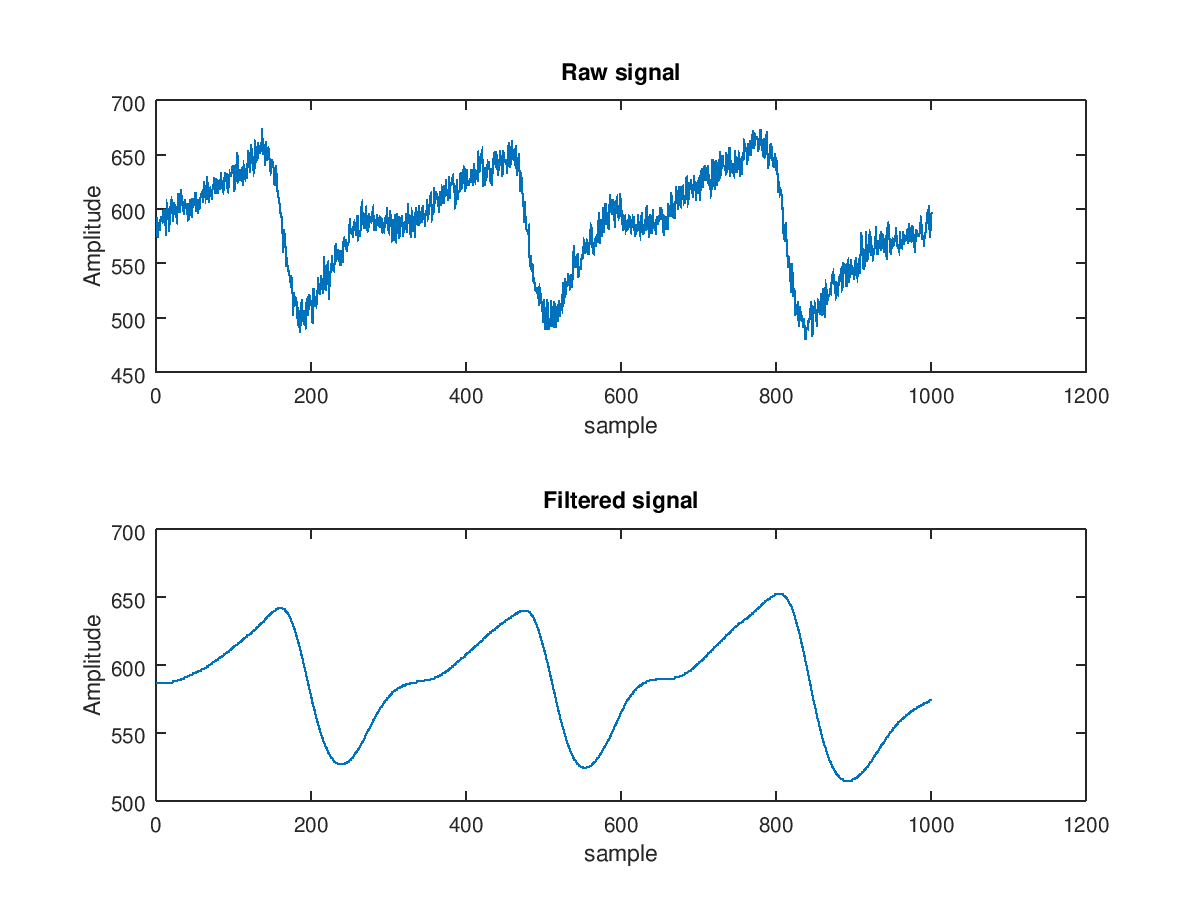
\includegraphics[width=0.75\textwidth]{../common/algo/filter.png}
			\caption{2\textsuperscript{nd} order butterworth IIR filter}
			\label{fig:filter}
		\end{figure}
		
		Octave's $butter$ function\footnote{\url{https://octave.sourceforge.io/signal/function/butter.html}} was used to get the transfer function coefficients for a low pass configuration. Sampling frequency of 500Hz and a cut-off 3.3Hz (for max HR of 200) was used. Calculated below are the coefficient values:
		
		$a_2 = -1.94137, a_3 = 0.94304$
		
		$b_1 = b_3 = 4.1762e-04$
		
		$b_2 = 8.3523e-04$
		
		To visualize filter's performance, a raw signal was captured from ADC, filter equation was implemented and applied on the input signal in Octave. As seen in Figure \ref{fig:filter} filter is quite effective in suppressing noise and produces a smooth output\footnote{Only a 1\textsuperscript{st} order filter was implemented in actual program as it worked "just fine", but it is much better to have a 2\textsuperscript{nd} order filter for suitable filtering performance.}.
		
	
	\subsection{Heart Rate}
	
		HR is calculated using mountaineer's method for peak detection (MMPD) in photoplethysmographic signals\cite{mmpd}.
		
		In this method, slope is calculated for every sample and as slope changes from positive to negative, sample will corresponding to a peak. Similarly a slope change from negative to positive would be a valley. A count for positive or negative consecutive slopes is also taken and compared with a preset value which updates with every detected peak to improve the robustness of the algorithm. A timer running would store peak timings and time difference between consecutive peaks would correspond to the heart rate. Shown below is a visualization of the algorithm ran on a sample set. Peaks \& valleys are captured quite accurately.
		
		\begin{figure}[ht!]
			\centering
			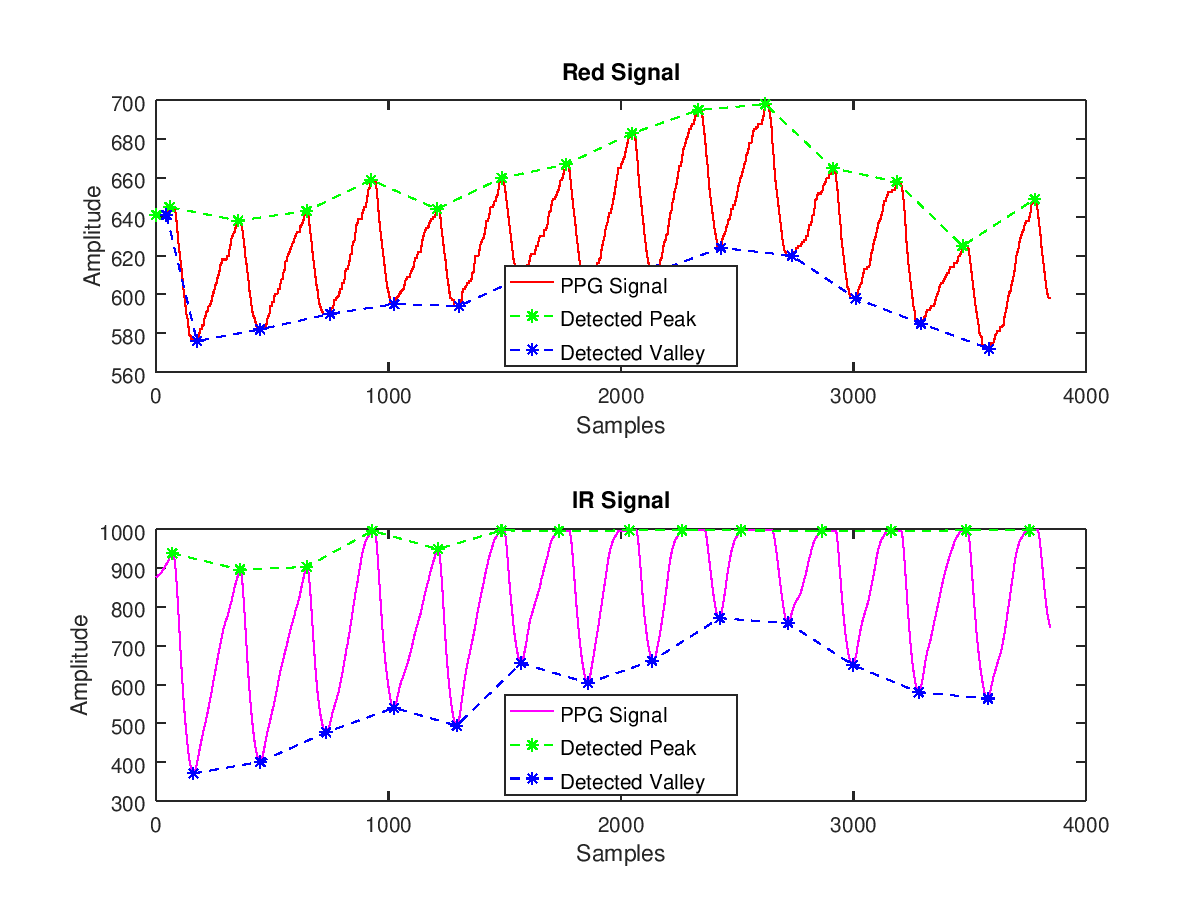
\includegraphics[width=0.7\textwidth]{../common/algo/mmpd.png}
			\caption{HR Algorithm applied to sample data}
		\end{figure}
	
	\subsection{SpO\textsubscript{2} Calculation}
		
		As discussed previously in equation \eqref{eq:calc}:
		
		
		\[
			R = \sfrac{\frac{V_{p2} - V_{l2}}{DC_2}}{\frac{V_{p1} - V_{l1}}{DC_1}}
		\]	
		
		We don't want to use signal's actual peak and valleys for R calculation as that is dependent on heart rate and any averaging of values on top of that would delay the final SpO\textsubscript{2}\% which we intend to obtain. Hence a weight averaging method is used\cite{wuk}, where instantaneous SpO\textsubscript{2}\% is calculated for neighboring samples and averaged together. This ensure multiple instantaneous values are obtained which can be averaged to obtain a final value. Following steps are performed in order:
				
		\begin{figure}[ht!]
			\centering
			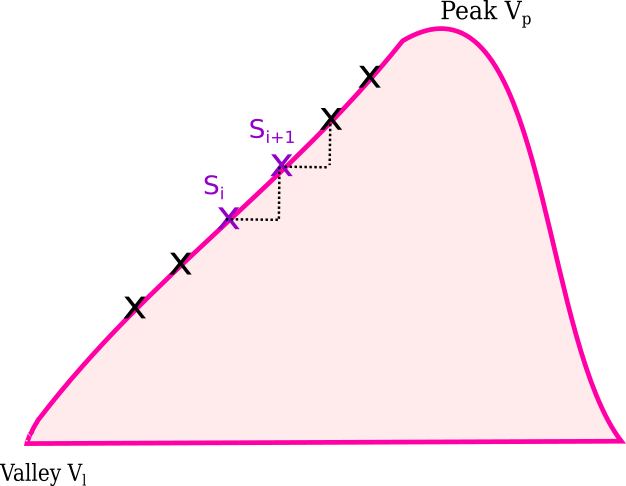
\includegraphics[width=0.5\textwidth]{images/spo2_algo.png}
			\caption{Selecting samples for instantaneous SpO\textsubscript{2}}
		\end{figure}
	
		\begin{enumerate}
			\item Find R between consecutive samples of red and ir signals: $S_{i+1}$ \& $S_{i}$. 
			
			\[
			R = \sfrac{\frac{S_{i_2+1} - S_{i2}}{DC_2}}{\frac{S_{i_1+1} - S_{i1}}{DC_1}}
			\]	
			
			Find SpO\textsubscript{2} with this R value which can obtained using a typical relationship curve equation as shown in Figure \ref{fig:curve}:
			\[		
				SpO_2 = -25*R + 110;
			\]
			\item Assign a weight to this SpO\textsubscript{2} based on the current average. If this instantaneous SpO\textsubscript{2} is lower than average, assign a lower weight. If nearer to average, assign a higher weight.
			
			\item Once weights are assigned for 20 samples, calculate a weighted average. Store this weighted average.
			
			\item Restart at step 1 and perform 10 such iterations.
			\item After 10 iterations, average the calculated weighted averages in each iteration. This becomes the final SpO\textsubscript{2}. Update this value with the current SpO\textsubscript{2} average which is used for assigning weights.
		\end{enumerate}
			
		A detailed explanation of this algorithm is in - Pulse Oximetry: Analysis of Theory, Technology and Practise\cite{wuk}
		
		Finally, an OLED display is refreshed every 5 secs with SpO\textsubscript{2}\% \& HR value.
		
